\documentclass[a4paper,12pt]{article}
\usepackage[margin=0.7in]{geometry}
\usepackage{tikz}
\usepackage{float}
\usepackage{pdflscape}
\usetikzlibrary{positioning,arrows.meta,shapes.geometric,fit,calc}
\begin{document}

\section*{Qt GUI Architecture (Conceptual)}
\begin{figure}[H]\centering
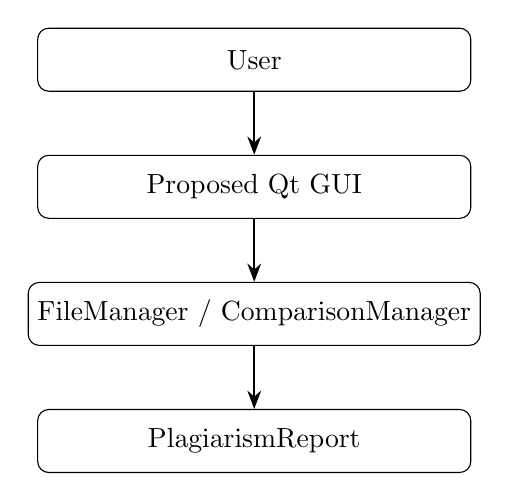
\begin{tikzpicture}[node distance=8mm, every node/.style={draw,rounded corners,align=center,minimum width=5.5cm,minimum height=8mm}, flow/.style={-{Stealth},thick}]
\node (n0) {User};
\node (n1) [below=of n0] {Proposed Qt GUI};
\node (n2) [below=of n1] {FileManager / ComparisonManager};
\node (n3) [below=of n2] {PlagiarismReport};
\draw[flow] (n0)--(n1);
\draw[flow] (n1)--(n2);
\draw[flow] (n2)--(n3);
\end{tikzpicture}
\textit{Conceptual only: Qt GUI was not found in the supplied source.}
\caption{Qt GUI Architecture (Conceptual) workflow.}\end{figure}
\end{document}
